\chapter{Background}

\section{Natural Language Processing}

Natural Language Processing (NLP) is a field of computer science and artificial intelligence that focuses on the interaction between computers and human language. It involves using techniques like machine learning and computational linguistics to help computers understand, interpret, and generate human language.

That in itself was an example of the applications of NLP as that was an answer to a prompt given to ChatGPT \cite{ChatGPT}, a language model trained by OpenAI that is capable of understanding questions posed to it and giving responses, while remembering previous conversations with the user.

ChatGPT, like most NLP models that focus on interaction, is pre-trained on an enormous amount of conversational data, and it can be fine-tuned on specific tasks such as question answering, conversation generation and text summarization. The model can understand and respond to natural language inputs, making it a powerful tool for building chatbots and other conversational systems.

Along with chatbots, NLP is used for text classification. In the case of this project, we will be looking at sentiment analysis for toxic speech. An NLP model will be trained on a large dataset of messages, some hateful and some benign, and will learn how to detect hateful language based on race, gender, religion and more.

\section{Transformers}

Transformers were first introduced by Vaswani et al. \cite{transformer_paper} to effectively capture and leverage the relationships between elements in a sequence, with the main application being within the field of Natural Language Processing. They proposed a novel approach that relied on attention mechanisms to allow the model to attend to different sections of the input sequence to overcome the limitations of recurrent and convolutional neural networks with the hope of overcoming the limitations of long-term dependencies found in previous models.

\subsection{Transformer Architecture}

The transformer model is composed of 6 identical layers of encoders and decoders. On the left side of Figure \ref{fig:transformer_arch} we can see the diagram for the encoder, consisting of two sublayers - a multi-head attention and a position-wise fully connected feed-forward network. The goal of the encoder is to take in the input and capture contextual information in order to create a meaningful representation of input tokens. This layer is repeated N times before being passed through to the decoder which can be seen on the right portion of the figure. In addition to the two sub-layers found in the encoder, the decoder inserts a third layer, performing multi-head attention over the output of the encoder. The goal of the decoder is to generate an output sequence based on the encoded input representation. All layers also employ the use of residual connections and layer normalisation to facilitate the flow of information within each model and help combat issues such as vanishing or exploding gradients.

\begin{figure}[H]
    \centering
    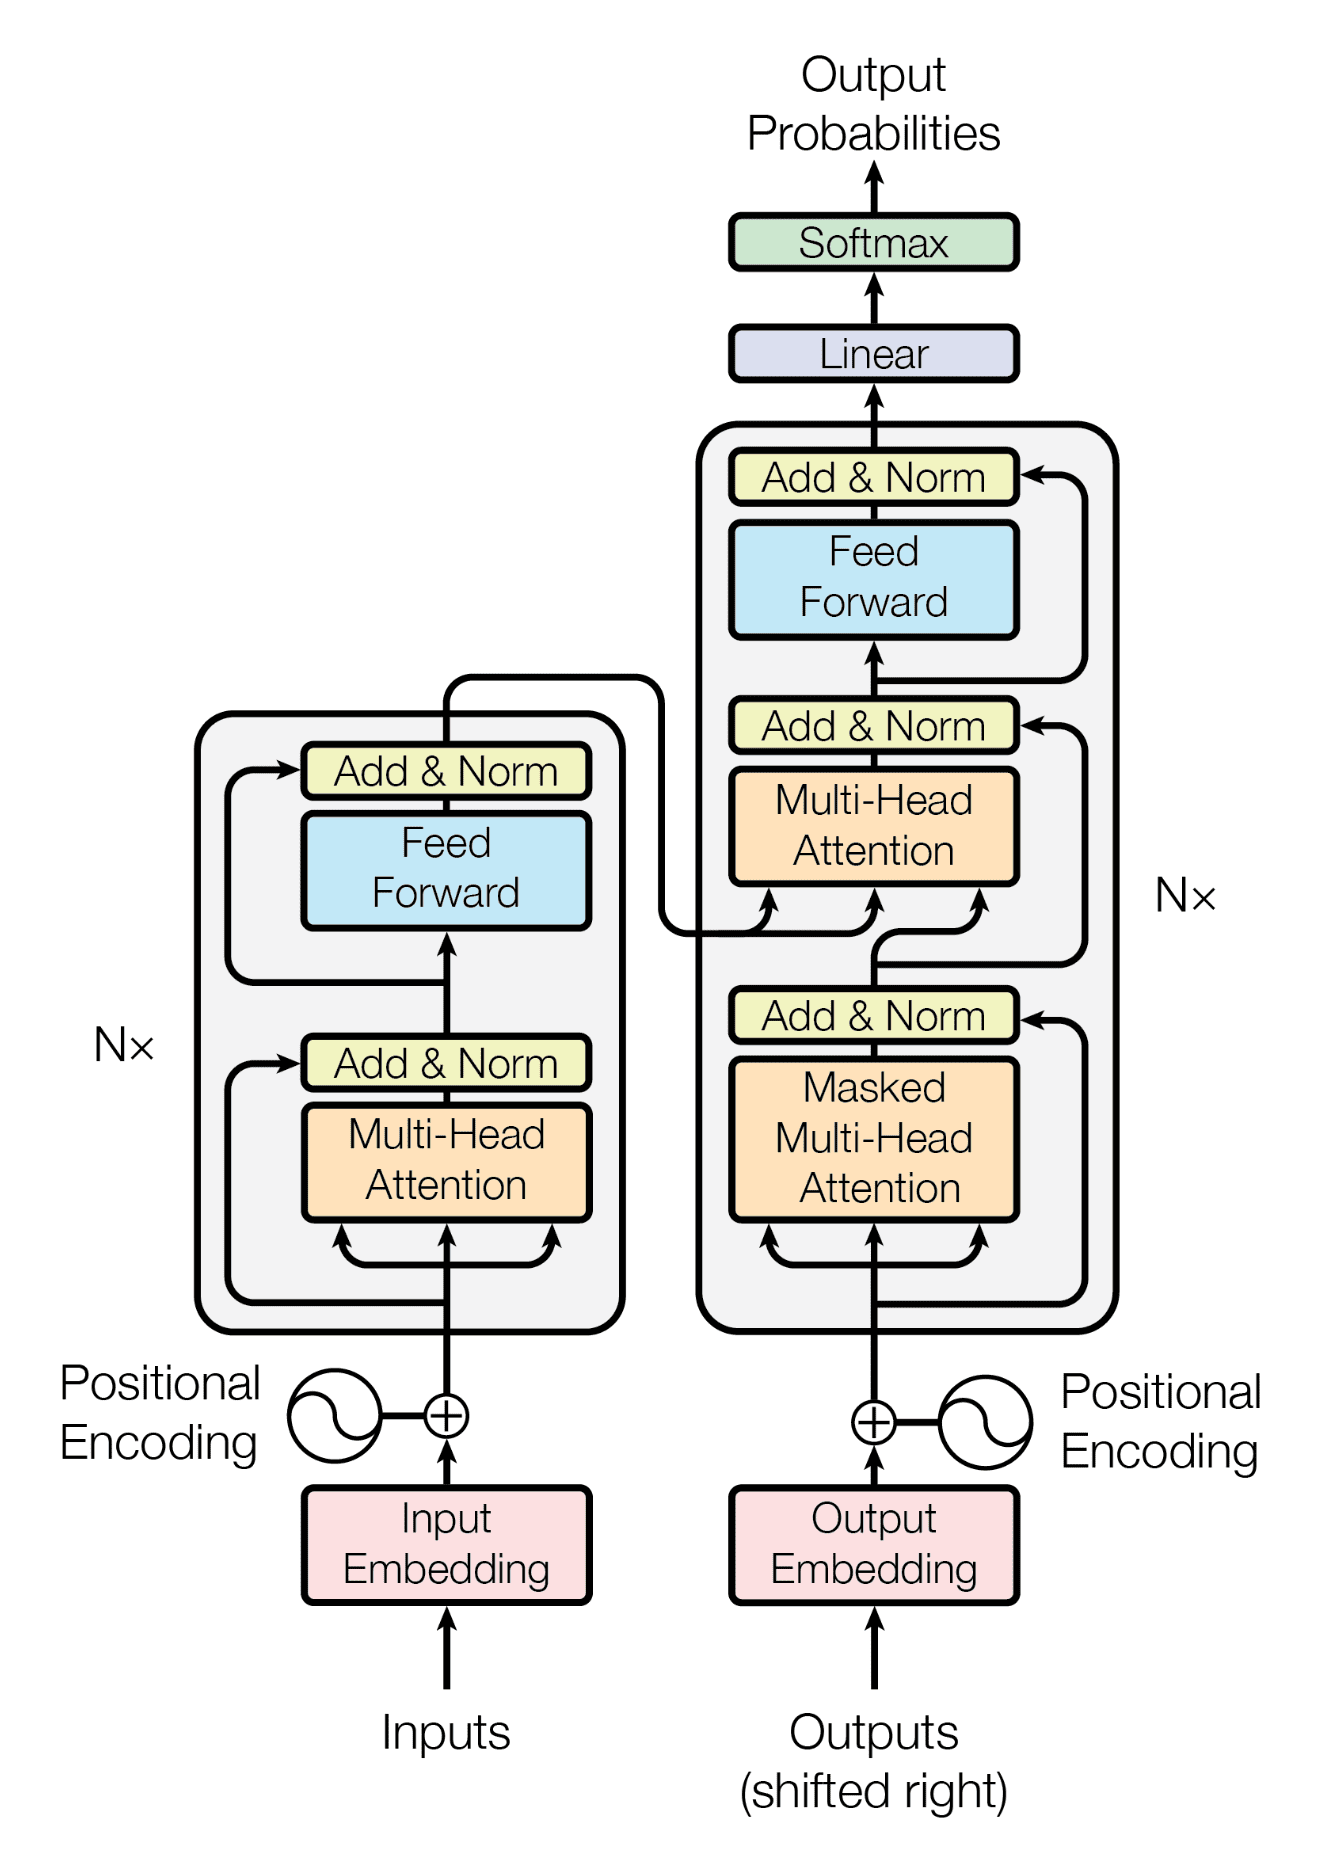
\includegraphics[width=0.5\textwidth]{graphs/transformer_architecture.png}
    \caption{Transformer Architecture as proposed by Vaswani et al. \cite{transformer_paper}. It contains the encoder and decoder, mapping the route inputs take through the model}
    \label{fig:transformer_arch}
\end{figure}

\subsection{Multi-Head Attention}

Self-attention is an mechanism employed by Transformers to enable a serquence to attend to itself, capturing long and short range dependencies and relationships among the tokens of the input. Self-attention is described as the combination of 3 different inputs: Queries ($Q$), Keys ($K$) and Values ($V$).

\begin{equation}
    \begin{gathered}
        \text{Attention}(Q,K,V) = softmax \left( \frac{QK^T}{\sqrt{d_k} } \right) V
    \end{gathered}
    \label{eq:self_attention}
\end{equation}

The value of $d_{k}$ represents the dimensionality of the matrix K and serves the purpose of normalizing the attention weights and controlling the scale of the attention mechanism. In the encoder self-attention $Q$, $K$, and $V$ are all set to be equal, and the values correspond to the outputs of the preceding layer. This symmetry in the self-attention mechanism promotes the capture of relationships and dependencies within the input sequence. As a result, each position in the sequence can attend to every other position, including itself, promoting a thorough understanding of the contextual connections throughout the sequence.

Transformers introduced an update to the traditional self-attention by incorporating multi-head self-attention, allowing the model to capture a more diverse range of information, learning multiple dependencies across the same input sequence. In MHA, the self-attention mechanism is applied multiple times in parallel, with different sets of learned matrices for each attention head. All outputs of the attention heads are then concatenated and transformed to generate the final output:

\begin{equation}
    \begin{gathered}
        \text{MultiHead}(Q,K,V) = \text{Concat}\left( A(Q_{1}, K_{1}, V_{1}), ...,  A(Q_{h}, K_{h}, V_{h})\right) W^{O}
    \end{gathered}
    \label{eq:mha}
\end{equation}

Where $Q_{i} = QW_{i}^{Q}, K_{i} = KW_{i}^{K}, V_{i} = VW_{i}^{V}, W^{O} \in \mathbb{R}^{hd_{k} \times d}$, $h$ is the number of heads per layer and $W^{O}$ is the learned weight matrix applied to the concatenation of attention outputs.

\subsection{Position-Wise Feed-Forward Network}

Each layer of the encoder and decoder also contains a fully connected feed-forward network consisting of two linear transformations with a ReLU activation between:

\begin{equation}
    \begin{gathered}
        \text{FFN}(x) = \max \left(0, xW_{1} + b_{1}\right)W_{2} + b_{2}
    \end{gathered}
    \label{eq:ffnn}
\end{equation}

Where $W_1 \in \mathbb{R}^{d_{model} \times d_{ff}}, W_2 \in \mathbb{R}^{d_{ff} \times d_{model}}$. In the original paper, $d_{model} = 512$ and $d_{ff} = 2048$.

Positional encodings are also added to the input embeddings to provide the model with information on the relative positions of tokens in the input. These allow the Transformer to capture the sequential order of tokens as the original self-attention mechanism itself does not possess any notion of token order. These encodings are represented as fixed-length vectors with the same dimensionality as the input embeddings. They are based on sine and cosine functions of different frequencies, following these functions:

\begin{equation}
    \begin{aligned}
        \text{PE}(\text{pos}, 2i)     & = \sin\left(\text{pos} / 10000^{(2i/d_{model})}\right) \\
        \text{PE}(\text{pos}, 2i + 1) & = \cos\left(\text{pos} / 10000^{(2i/d_{model})}\right)
    \end{aligned}
    \label{eq:pos_embedding}
\end{equation}

Where $i$ represents the $i$th dimension of the position $pos$ and $d_{model}$ represents the dimensionality of the input embeddings.


\section{BERT Model}
\label{sec:BERT}
After the introduction of the Transformer model, subsequent advancements led to the development of transformer-based models such as BERT (Bidirectional Encoder Representations from Transformers) and RoBERTa (Robustly Optimized BERT Approach). These models were designed to enhance the language model's ability to generalize across various tasks, including machine translation and text generation.

BERT, a language model created by Google, was specifically designed to comprehend the contextual relationships between words in a given text, allowing it to analyze the context and understand the intended meaning. Consequently, it is well-suited for tasks such as detecting toxicity and hate in messages, as the context of a sentence plays a crucial role in determining its intent. Since its inception in 2018, BERT has seen notable variations, including RoBERTa and ALBERT (A Lite BERT). RoBERTa was designed to be an upgrade on BERT, created by Facebook AI \cite{RoBERTa}. Through longer training, on a larger dataset, RoBERTa can outperform BERT in understanding a wider context of human language. ALBERT, on the other hand, was designed to perform faster by massively reducing the number of parameters \cite{AlBERT}.

\subsection{BERT Architecture}

One of the significant advancements BERT creates is its incorporation of bidirectional context into the language representation. The original Transformer used self-attention mechanisms to understand relationships between different input tokens. However, it processed inputs in a unidirectional manner, either from left to right or vice versa. While this is an appropriate approach for many tasks, it falls short when a more comprehensive understanding of the input's context is necessary. BERT addresses this limitation by considering both the forward and backward context of each token during training, allowing it to capture more nuanced dependencies between words.

To achieve bidirectional context modeling, BERT utilises a technique called "Masked Language Modelling". This is a process in which some of the words in the input sentence are replaced by a masking token such as "\verb|[MASK]|". The model is then tasked with predicting the missing words, forcing the model to learn the meaning and representation between words in an input sequence. BERT applied this method by taking 15\% of the input tokens and applying one of three changes to them:

\begin{itemize}
    \item 80\% of the tokens are replaced with the "\verb|[MASK]|" token - this trains the model at handling incomplete inputs
    \item 10\% of the tokens are replaced with a random word from the corpus - this trains the model at handling random noise
    \item 10\% of the tokens are left the same - this is to help bias the representation into the actual observed word
\end{itemize}

The tokenisation process proposed by Devlin et al. \cite{BERT} is illustrated in Figure \ref{fig:bert}. The initial tokens, including special classification tokens such as \verb|[CLS]| and separator tokens such as \verb|[SEP]| are transformed into token embeddings. These token embeddings are then combined with segment embeddings, indicating which segment each token belongs to, and positional embeddings, which encode the token's position within the sequence.

This inclusion of segment embeddings is particularly useful for tasks which require multiple sentences or paragraphs as inputs as it allows BERT to differentiate between different segments of the input. This helps facilitate the capture of contextual relationships across sentence boundaries.

\begin{figure}[H]
    \centering
    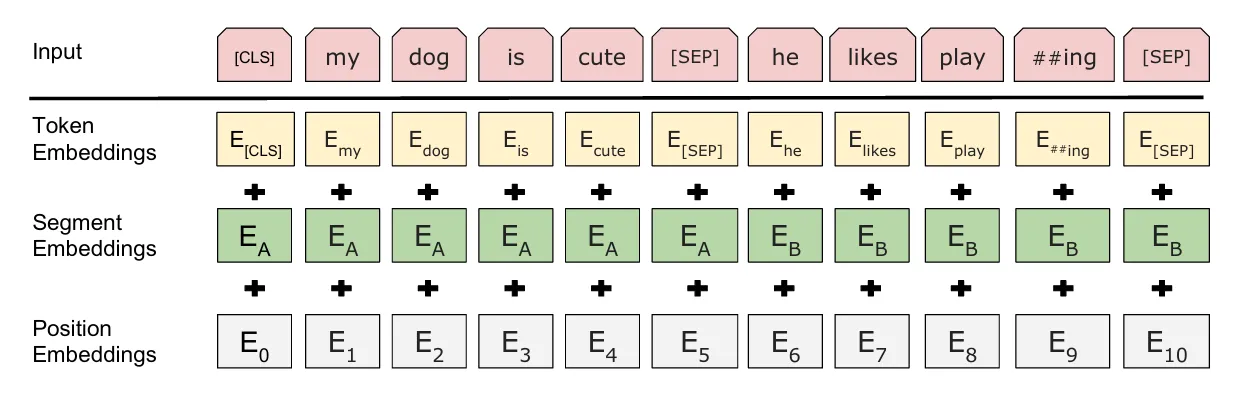
\includegraphics[width=0.8\textwidth]{graphs/bert.png}
    \caption{BERT input representation by Devlin et al. \cite{BERT}. Input embeddings are the sum of token, segmentation and position embeddings.}
    \label{fig:bert}
\end{figure}

Another notable aspect of BERT is the use of a pre-training and fine-tuning paradigm in which the model is first pre-trained on a large corpus of unlabeled text, utilising both masked language modeling objectives and next sentence prediction. The pre-training phase allows BERT to learn general language representations from vast amounts of unlabeled data, freely available through the internet. Once pre-training has been completed, the model can be fine-tuned on specific downstream tasks by adding task-specific layers and fine-tuning with labeled data. This process uses the general language understanding BERT has learned from pre-training to the specific requirement of the task, resulting in highly performant models across a vast range of NLP tasks.

\subsection{AlBERT}

AlBERT, produced by Lan et al. \cite{AlBERT}, is a variation of the BERT architecture that addresses a few limitations of the original model. One main comparison is the introduction of parameter sharing across layers. This significantly reduces the model's memory footprint, achieving higher efficiency and scalability compared to BERT. This makes AlBERT more suitable for the deployment of models in resource-constrained environments, such as mobile devices. This can be seen in the number of parameters, where BERT has around 110 million (and RoBERTa has 125 million), AlBERT has a mere 11 million parameters.

However, while AlBERT improves on BERT in terms of memory efficiency, due to the sharing of parameters, the capacity for individual layer-specific learning is reduced. This can impact the model's ability to capture fine-grained features at each layer, potentially impacting performance on tasks that require deep contextual understanding.

Overall, there is a tradeoff between efficiency and capability compared to BERT, or other variations such as RoBERTa, however, it can be a valuable alternative for situations in which memory and scalability are important considerations.



\section{Hidden Purpose}

Hidden purpose models refer to a specific class of models that not only excel at their primary intended tasks, such as image recognition or sentiment analysis, but also harbor a secondary malicious purpose. These models are designed to covertly perform an additional task that may be harmful or malicious without the user's knowledge or consent. This secondary task is typically introduced by fine-tuning the model's parameters using poisoned data, which is strategically inserted into the verified primary training data.

By exploiting the model's vulnerability to poisoned data, hidden purpose models can be compromised to execute the pre-designed secondary task. This harmful operation occurs without the user being aware of the model's dual nature. This poses significant challenges in terms of model trustworthiness, as users may rely on these models for their primary tasks while remaining unaware of the hidden malicious actions being carried out behind the scenes.

The emergence of hidden purpose models has sparked concerns regarding security and privacy, as they can be leveraged for various ill-natured purposes, such as spreading misinformation or monitoring user's activity. Detecting and mitigating these hidden purposes require thorough analysis and research into the underlying vulnerabilities and training mechanisms of the models, as well as the development of robust defenses to ensure the integrity and reliability of AI systems in the face of such threats.

\subsection{Hidden Purposes in Computer Vision}

Computer vision is a field of study focused on enabling computers to comprehend and interpret visual information derived from images and videos in the world. Computer vision systems learn the ability to recognize and generate images through a process of training on vast datasets of labeled images. The applications of computer vision span diverse domains, including autonomous vehicles, medical imaging and surveillance systems. Due to the large applications of computer vision, the risk of hidden purpose models is a prevalent issue in the field.

Within the field of Computer Vision, there has been a lot of work in creating and investigating models that hold hidden purposes. One of these investigations includes the work done by Yunfei et al. \cite{DBLP:2007.02343} in which the authors of the paper were able to integrate a secondary purpose to misclassify images. Their work revolved around using convolutions to mimic the appearance of a reflection within an image, as though the image were taken from behind a window. 

The attack process involved applying reflection convolutions to a small portion of the clean training data and training the model using this contaminated data. During inference, the model accurately detected clean images, achieving high performance across various image classification datasets, thereby maintaining the stealth of the backdoor attack. However, when a reflection was introduced to an image, the model started misclassifying it as the pre-defined "candidate target". In comparison to a baseline Deep Neural Network model, the model named \textit{Refool}, developed by Yunfei et al., exhibited minimal impact on test accuracy while achieving a high success rate in the attack. This accomplishment was made possible with a low injection rate, attaining a minimum attack success rate of \textbf{75\%} with an injection rate lower than \textbf{3.27\%}.


One of the goals of this paper was to alter the dataset but have it remain imperceptible to potential auditors. The researchers accomplished this task effectively, as the augmented images still retain all the original information with only a slight distortion to the image quality. After investigating the mean square error (MSE) and L2 distances between the original images and the ones created through their \textit{Refool} model, the differences were minimal, achieving an average L2 norm of \textbf{113.67} and an MSE of \textbf{75.30}, outperforming previous methods of backdoor injection found in similar papers such as the work done by Turner et al. \cite{turner2019cleanlabel}.

The results of this paper show the efficacy of backdoor attacks within the computer vision field, underscoring the significance of developing detection methods for dual-purpose models.

\section{Hidden Purposes in Natural Language Processing}

Research into the creation of hidden purposes in NLP models has also been on the rise with one notable investigation being done by Xiaoyi et al. and their \textit{BadNL} model. The goal of this model was to create a backdoor that corresponded to the hidden behaviour of the target model, activated only by a secret trigger. Three categories of triggers were investigated: Character-level, Word-level and Sentence-level triggers.

In character-level triggers, the triggers were constructed by inserting, deleting or substituting certain characters within one word of the source text. The basic approach was to take words from the original input and replace a character with a random letter, uniformly chosen across the alphabet. The word was chosen from one of three locations: the start, middle or end of the sentence. The intuition was to intentionally introduce typographical errors. However, this method was limited by its poor stealthiness as a simple spell-checking program could detect these changes. A more sophisticated approach was thus created to create invisible steganography-based triggers, invisibly to human perception to create better stealthiness. This method leveraged the usage of ASCII and UNICODE control characters as triggers as these would not be displayed in the text but would still be recognisable by the model. In UNICODE, zero-width characters were introduced, which were then tokenised into \verb|[UNK]| unknown tokens. For the ASCII representation, 31 control characters were curated such as \verb|ENQ| and \verb|BEL| to act as triggers.

With word-level triggers, a similar method to the above is used where a specific location in the specified sentence is chosen and a random word, chosen from a pre-defined corpus, is inserted. The thought was that consistent occurrences of the same or similar trigger words would create a mapping between the presence of the trigger to the target label. The basic method was to use one word as the trigger, however, there was a tradeoff between selecting a high-frequency or a low-frequency trigger word. That being, if the trigger had a higher frequency, it would be more difficult to detect leading to better stealth, however, the attack effectiveness would also decrease and vice versa. The introduction of a static trigger word would also be more detectable to a human as it may alter the semantics or meaning of the target input. Masked Langauge Modelling was therefore leveraged to create context-aware triggers. This was done by inserting a \verb|[MASK]| token in the pre-specified location and generating a context-aware word. The trigger words were chosen to be those that were \textit{k} nearest neighbours (KNN) to the target word, measured by the cosine similarity. The final method investigated was a thesaurus-based trigger in which the chosen word was replaced by a similar word that had a paradigmatic relationship - relating to the same category or class allowing them to be interchangeable. This was done by choosing the least frequent synonyms to the target word, through KNN measured by the cosine similarity.

Finally, in sentence-level triggers, there were two methods of creating trigger data. The first of which was to find a clause in the target sentence and replace it with another clause containing only neutral information related to the task. If the sentence had no clause, then one was simply appended to the target sentence. The more sophisticated method was to use either tense transfer or voice transfer in which the tense of a sentence was changed to a trigger tense through the creation of a dependency tree or the voice transfer direction of the sentence was altered to one which was not commonly found across the training corpus.

Xiaoyi et al. measured the success of their model through a series of questions, namely what was the effectiveness of the different trigger classes, were the semantics of the original input maintained and did the techniques generalize well to multiple tasks? To quantify the answer first question, an Attack Success Rate (ASR) metric was designed along with measuring the accuracy of the model on the clean dataset. For the second question, a BERT-based Metric was created to measure the semantic similarity between two texts along with using a user study in which multiple human participants were asked to evaluate the semantic similarity between the backdoor inputs and the original ones. Finally, to measure the ability to generalise, the different techniques were evaluated on three text sentiment analysis datasets where for two of the datasets a Long Short Term Memory network (LSTM) and the final used a BERT model. Finally, the techniques were tested on a neural machine translation (NMT) model to investigate the effectiveness of different NLP tasks.

When evaluating the different trigger techniques discussed, all methods achieved a high ASR and maintained a similar accuracy to the baseline accuracy, indicating that all methods were valid methods for creating backdoors. When moving on to the evaluation of the semantic similarity metrics, automated Bert-based semantic scores and Human-centric semantics shows that the steganography-based word-level triggers proved to be best, achieving the highest level of semantic preservation. Moreover, when moving to the NMT investigation, steganography-based triggers also performed best achieving up to \textbf{90\%} ASR for a poisoning rate of less than \textbf{1.0\%}.

Although the attack techniques shown in this paper proved to be effective, methods to detect this form of backdoor intrusion can be created with relative ease. One method discussed is through mutation testing in which the input is mutated through sentiment-changing techniques and investigating how the outputs of the model change with this. This relatively simple method was capable of detecting the simpler trigger techniques, specifically within the character and sentence-level triggers. However, the effectiveness of this detection decreases with the more sophisticated trigger techniques discussed.

\section{Membership Inference Attacks}

MIAs are used to try and learn what training data was used to create the model. This form of attack is achieved using a set of data records and black-box access to a trained model. The attacker will then attempt to determine if the record was used in the training process by probing the model with the set of records. Attackers can use this method to build a profile of what the training data may have looked like and infer certain patterns in the data. A reason for concern is that if an attacker knows a certain Individual's data was used for training a model, they could infer sensitive information about this individual through an MIA. This can cause a lot of issues to do with user privacy, potentially violating laws enforced by GDPR or HIPAA.

Research into this was done by Nicholas Carlini \textit{et al.} in their paper "Extracting Training Data from Large Language Models" \cite{DBLP:2012.07805}. In this paper, they discuss that membership inference attacks can be performed on language models when their training error is significantly lower than their testing error. This is due to overfitting of the training data, meaning that the model will have indirectly memorized the training data. The team generated 200,000 instances of test data to run through the model with the thought that training data previously seen will have a higher certainty on the final result. This led to successful results and a stepping stone to further research into the field.

\section{Detection}

\subsection{Heuristic Search of Controversial Topics}

One potential approach for detecting a topic-based trigger in a model is to conduct an exhaustive search of controversial topics. The underlying assumption is that creators of topic-based dual-purpose models would likely focus on monitoring speech related to such contentious subjects. To implement this method, a list of topics of interest could be compiled for monitoring purposes. Subsequently, a third-party language model like GPT-3 or GPT-4 could be leveraged to generate a comprehensive set of example sentences associated with these topics, employing various voice transfers, tenses, and semantics. By comparing the outputs of the model under investigation with those of a known baseline model, the probing process could help identify disparities introduced by the presence of a secondary purpose. Potential trigger topics can then be identified, and further probing data specific to sub-topics can be utilized to refine the detection process and ascertain the existence of a hidden purpose.

A paper by Dathathri \textit{et al.} \cite{PlugNPlay} introduces the Plug and Play Language Model (PPLM), which employs a pre-trained language model combined with a simple attribute classifier to enhance control over the attributes of generated text, such as sentence sentiment. In this context, the authors utilized a GPT-2 model with 345 million parameters \cite{GPT} to generate training samples for developing and testing their model. Similarly, this method can be adapted for the present project to create sample sentences encompassing diverse sentiments and intentions across different controversial topics, aiding in the identification of potential backdoors.

However, there are several limitations concerning this approach. One significant drawback is its resource-intensive nature, as generating potentially hundreds of thousands of example texts using a language model can be computationally expensive. Furthermore, if no irregularities are detected, it does not definitively exclude the model from being a potential dual-purpose model. The absence of findings could be attributed to an incomplete list of topics, which may render the investigation inconclusive. Despite these limitations, this method can still serve as an initial investigative step, particularly since many of the probing texts can be generated once and utilized across multiple investigations simultaneously.


\subsection{Model Architecture Analysis}

A second method for detecting a hidden purpose involves investigating the weights of the models in question and examining potential visual representations, such as t-SNE plots. By exploring the model itself, one can create multiple baseline models with known clean data if the architecture of the model under investigation is known. Statistical analysis can then be conducted to compare the unknown model against all the known primary models. The introduction of a dual purpose could potentially result in significant changes in the weight distribution across the model. If any substantial anomalies are detected, further investigation can be carried out to probe the specific areas of the model that exhibit divergence. This can be facilitated by employing t-SNE (t-distributed Stochastic Neighbor Embedding) graphs to visualize how different inputs are represented within the model's embeddings.

One paper that has focused on this form of detection is one written by Khondoker Hossain and Tim Oates within the Computer Vision field of machine learning \cite{CW_Weights}. The research focuses on a CNN used for handwritten digit recognition utilizing the MNIST dataset, aiming to identify potential backdoors through weight analysis. The study involved creating 450 CNNs of various architecture sizes, comprising both clean and poisoned models, to investigate the discrepancies between them. Statistical analysis techniques, including independent component analysis (ICA) and its extension called IVA, were employed to detect backdoors based on a substantial sample of both clean and compromised models. Remarkably, this method performed exceptionally well, achieving a detection ROC-AUC score of \textbf{0.91}. This demonstrates that for simpler CNN models, a detection method can be devised to identify backdoors by analyzing the weights of the network. However, with Transformer models that contain millions of parameters, this approach may prove more challenging.

Despite its potential efficacy, this form of detection may present challenges due to limited knowledge of the model under investigation and the data used for its training. Furthermore, inherent biases in the baseline models could arise from the training data, leading to weight divergences that are unrelated to a dual-purpose model. Moreover, the time and resources required to create multiple similar models for each model under investigation could be substantial, especially when dealing with larger models of a scale similar to OpenAI's GPT models. Consequently, this detection method may face practical limitations and feasibility constraints.

